\documentclass{standalone}

\usepackage{amsmath,amssymb,physics,bm}
\usepackage{tikz}
\usetikzlibrary{%
	calc,
	patterns,
	positioning,
	decorations.pathreplacing,%
	decorations.pathmorphing,%
	arrows.meta,%
}
\usepackage{bamcolors}

%\usepackage[active, tightpage]{preview}
%\PreviewEnvironment{tikzpicture}
%\setlength\PreviewBorder{2mm}

\begin{document}
\begin{tikzpicture}
    \pgfmathsetmacro\w{5}% width
    \pgfmathsetmacro\h{0.6 * \w}% height
    \pgfmathsetmacro\Nx{10}
    \pgfmathsetmacro\Ny{0.5 * \Nx}

    % fill oversampling domain before drawing the grid
    \draw[fill=BAMgrad020] (3 * \w / \Nx, 1 * \h / \Ny) rectangle ++(3 * \w / \Nx, 3 * \h / \Ny);

    % coarse grid color
    \def\cc{BAMgrad080}
    % vertical lines
    \foreach \x in {0, 1, 2, ..., \Nx}{
        \draw[\cc] (\x / \Nx * \w, 0.0)--(\x / \Nx * \w, \h);
    }
    % horizontal lines
    \foreach \y in {0, 1, 2, ..., \Ny}{
        \draw[\cc] (0, \y / \Ny * \h)--(\w, \y / \Ny * \h);
    }
    % draw rectangle in black
    \draw[BAMgrad100] (0, 0) rectangle (\w, \h);

    % draw oversampling domain boundary
    \draw[draw=BAMred2] (3 * \w / \Nx, 1 * \h / \Ny) coordinate (S) rectangle ++(3 * \w / \Nx, 3 * \h / \Ny);
    % annotate subdomain
    \path (S) ++(3 * \w / \Nx / 2, 2.5 * \w / \Ny /3) coordinate (Scenter);
    \node at (Scenter) {$\varOmega_i^{\bm\mu}$};
    \node[below = 0.2 mm of S] {\textcolor{BAMred2}{$\varGamma^{\bm\mu}_{\mathrm{out}}$}};

    % dirichlet boundary
    \draw[BAMblue2, thick] (0, 0) -- (0, \h);
    \coordinate (D) at (0, 0.5 * \h);
    \node[left = 2mm of D] {$\varSigma^{\bm\mu}_{\mathrm{D}}$};
    % neumann boundary
    \draw[BAMred2, thick] (\w, 0) -- (\w, \h);
    \coordinate (N) at (\w, 0.5 * \h);
    \node[right = 2mm of N] {$\varSigma^{\bm\mu}_{\mathrm{N}}$};

    % draw dashed rectangle to indicate the zoom
    \draw[dashed,BAMgrad080] (9 * \w / \Nx - 0.05, -0.05) -- ++(\w/\Nx + 0.1, 0) coordinate (A) -- ++(0, \h/\Ny+0.1) -- ++(-\w/\Nx-0.1, 0) -- cycle;

    % arrow from cell to unit cell mesh
    \node[] (1) at (\w-\w/\Nx/2, \h/\Ny/2) {};
    \path (1) ++(3cm, 1cm) coordinate (2);
    \node[inner sep=0pt] (unit cell) at (2) {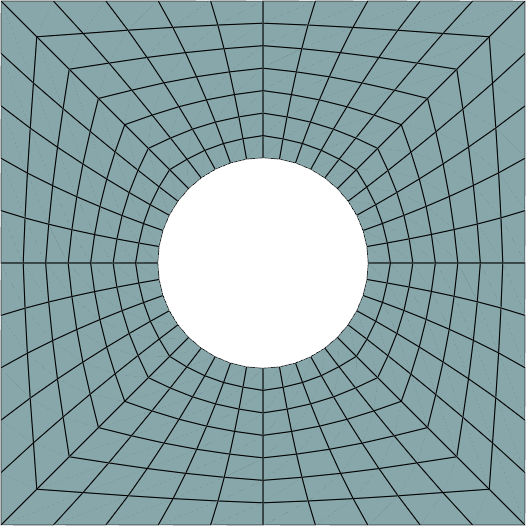
\includegraphics[keepaspectratio,width=2.25cm]{unit_cell.png}};
    \path[thick,-stealth, BAMgrad080] (A) edge[bend right] node [below] {} (unit cell);
    % (a), (b) identifier for figure
    \node[below = 4mm, inner sep=0] at (\w/2, 0) {(a)};
    \node[below = 5mm of unit cell, inner sep=0] {(b)};
\end{tikzpicture}
\end{document}
